\documentclass[tikz,border=4pt]{standalone}
% Estilos compartilhados pelos diagramas dos estágios e módulos do Core.
\usetikzlibrary{arrows.meta, positioning, calc, shapes.geometric, fit}

\tikzset{
  >={Stealth[length=2.2mm]},
  bloco/.style={draw, rounded corners=2pt, minimum width=24mm, minimum height=9mm,
                align=center, font=\small, fill=blue!6},
  regpipe/.style={draw, minimum width=9mm, minimum height=48mm, align=center,
                  font=\small, fill=gray!25},
  mux/.style={draw, trapezium, trapezium angle=70, shape border rotate=90,
              minimum height=11mm, minimum width=7mm, inner sep=1pt, align=center,
              font=\scriptsize, fill=orange!15},
  ctrl/.style={draw, rounded corners=2pt, minimum width=24mm, minimum height=9mm,
               align=center, font=\small, fill=green!10},
  opcional/.style={bloco, dashed, fill=yellow!12},
  externo/.style={draw, rounded corners=2pt, minimum width=24mm, minimum height=9mm,
                  align=center, font=\small, fill=red!8},
  dado/.style={->, thick},
  sinal/.style={->, dashed},
  rotulo/.style={font=\scriptsize, midway, above, inner sep=1pt},
  titulo/.style={font=\bfseries\normalsize}
}

\begin{document}
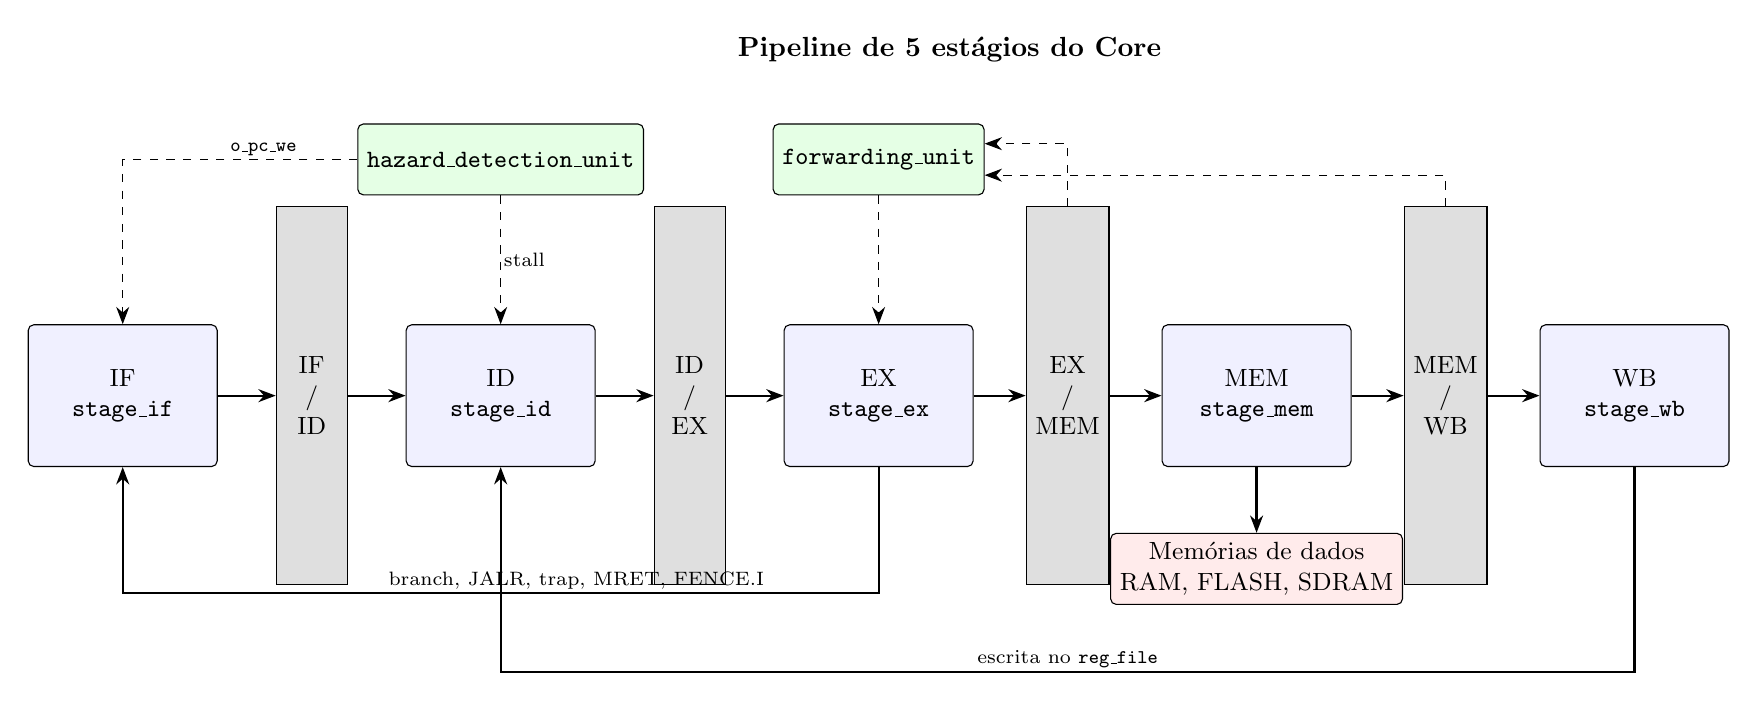
\begin{tikzpicture}
  \node[titulo] at (10.5,4.4) {Pipeline de 5 estágios do Core};
  \node[bloco, minimum height=18mm] (if) at (0,0) {IF\\\texttt{stage\_if}};
  \node[regpipe] (r1) at (2.4,0) {IF\\/\\ID};
  \node[bloco, minimum height=18mm] (id) at (4.8,0) {ID\\\texttt{stage\_id}};
  \node[regpipe] (r2) at (7.2,0) {ID\\/\\EX};
  \node[bloco, minimum height=18mm] (ex) at (9.6,0) {EX\\\texttt{stage\_ex}};
  \node[regpipe] (r3) at (12.0,0) {EX\\/\\MEM};
  \node[bloco, minimum height=18mm] (mem) at (14.4,0) {MEM\\\texttt{stage\_mem}};
  \node[regpipe] (r4) at (16.8,0) {MEM\\/\\WB};
  \node[bloco, minimum height=18mm] (wb) at (19.2,0) {WB\\\texttt{stage\_wb}};
  \foreach \a/\b in {if/r1, r1/id, id/r2, r2/ex, ex/r3, r3/mem, mem/r4, r4/wb}
    \draw[dado] (\a) -- (\b);

  \node[ctrl] (hdu) at (4.8,3.0) {\texttt{hazard\_detection\_unit}};
  \node[ctrl] (fwd) at (9.6,3.0) {\texttt{forwarding\_unit}};
  \draw[sinal] (hdu) -- node[rotulo, right] {stall} (id);
  \draw[sinal] (hdu.west) -| node[rotulo, pos=.2] {\texttt{o\_pc\_we}} (if.north);
  \draw[sinal] (fwd) -- (ex);

  \draw[dado] (ex.south) -- ++(0,-1.6) -| node[rotulo, pos=.2, above] {branch, JALR, trap, MRET, FENCE.I} (if.south);
  \draw[dado] (wb.south) -- ++(0,-2.6) -| node[rotulo, pos=.25, above] {escrita no \texttt{reg\_file}} (id.south);
  \draw[sinal] (r3.north) |- ([yshift=2mm]fwd.east);
  \draw[sinal] (r4.north) |- ([yshift=-2mm]fwd.east);
  \node[externo] (mm) at (14.4,-2.2) {Memórias de dados\\RAM, FLASH, SDRAM};
  \draw[dado] (mem.south) -- (mm.north);
\end{tikzpicture}
\end{document}
